\chapter{Estudio de Simulación}
El presente capítulo tiene como objetivo realizar un estudio de simulación en el que se evalúe el adecuado la adecuada estimación del modelo propuesto en los capítulos antecedentes. Esto comprende generar una base de datos en dónde se tenga una variable aleatoria $Y_i \sim W_r(q_t, \alpha,t)$, la cual está subyace la variable censurada $Z$ que sigue lo denotado en la sección 3.1. Asimismo, dicha base de datos contiene otras variables simuladas, las cuales actuarán como variables independientes en un contexto de regresión. El objetivo principal del estudio de simulación evaluar si el método de estimación planteado, permite recuperar adecuadamente los parámetros de regresión establecidos a priori. Los criterios sobre los cuales se analizará la estimación del modelo son: sesgo relativo, error cuadrático medio y cobertura.

El proceso de simulación consiste en generar 100 réplicas considerando tamaños de muestra de $n=\{10000\}$. Simularemos la variable respuesta $Y_{i} \sim W_r(Q_{t_{i}},\alpha,t)$ considerando 3 covariables $X_{1i},X_{2i},X_{3i}$ que serán simuladas como:
\[X_{1i} \sim Beta(2,3)\]
\[X_{2i} \sim Normal(2,0.5)\]
\[X_{3i} \sim Gamma(2,25)\]

Conforme lo mencionado en la sección 3.2.1, $q_{t_{i}} =  \exp(x_i^T \beta)$, en dónde $\beta =[0.5, 0.3, 0.6, 0.8]^T$ y $x_{i}=(1,X_{1i},X_{2i},X_{3i})^{T}$. Por otro lado, el parámetro de dispersión tomará el valor $\alpha = 2$. Finalmente, se realizará la evaluación por los cuantiles $t = [0.1, 0.2, \dots, 0.9]$.

Se asume que $Y_i \sim W_r(q_{ti}, \alpha,t)$ se observa con censura intervalar. En este estudio asumiremos que solo observamos una variable $Z$ que particiona la variable $Y_i$ en intervalos de igual amplitud, con la excepción del último intervalo, el cual tiene la estructura $[L_{inf}, \infty]$. Una vez generada dicha variable, se realiza el modelamiento de la variable con censura intervalar sobre las variables independientes creadas previamente. El objetivo final es, a través del modelo, estimar los coeficientes $\beta$ definidos previamente.

\section{Implementación del modelo}

La implementación del modelo se realizó a través del lenguaje de programación R, tomando en consideración las definiciones presentadas en el capítulo 3 de la presente tesis. El seudocódigo de la implementación es el siguiente:

\begin{lstlisting}
Simulamos n valores de las siguientes distribuciones:

X1 ~ Beta(2,3) 
X2 ~ Normal(2,0.5)
X3 ~ Gamma(2,25)

Definimos los siguientes valores:

B = [0.5, 0.3, 0.6, 0.8] 
Sigma = 2
Qt = exp(B[1] + B[2]*X1 + B[3]*X2 + B[4]*X3)
t=[0.1, 0.2, 0.3, 0.4, 0.5, 0.6, 0.7, 0.8, 0.9]
M = 5,000

Para cada cuantil en t:
	Para cada replica en M:
		1 Simular n valores de la distribucion 
			Y ~ W_r(Qt, Sigma, cuantil)
		2 Censurar la variable Y de forma intervalar tal que
			Z ~ Categorica
		3 Obtener los limites inferiores y superiores de
			cada categoria de Z
		4 Crear la base de datos simulada
			df <- [L_inf, L_sup, X1, X2, X3]
		5 Ejecutar la regresion de censura intervalar
		6 Guardar los resultados
\end{lstlisting}

% Pseudocódigo del modelo?

Una vez generadas las simulaciones, se evaluó para cada escenario (cuantil y tamaño de muestra) lo siguiente:
\[ \hat{\text{Sesgo relativo:}} \frac{1}{M}(\hat{\theta_j} - \theta)\]
\[ \hat{\text{ECM:} \frac{1}{M}} \sum_1^M (\hat{\theta_j} - \theta)^2 \]
\[ \hat{\text{Cobertura:} \frac{1}{M}} \sum_1^M (\hat{\theta_j} - \theta)^2 \]

\noindent dónde $\theta$ es el verdadero valor del parámetro, $\hat{\theta}_{j}$ la estimación obtenida en la j-ésima réplica y M el número de réplicas.

\section{Resultados}

En la tabla a continuación se muestra, para cada tamaño de muestra y parámetros $\Theta = [\beta_0,\beta_1,\beta_2,\beta_3,\sigma] = [0.5, 0.3, 0.6, 0.8, 2]$ los resultados de las métricas utilizadas para evaluar el desempeño de los estimadores bajo la estructura propuesta. Para las 100 réplicas identificadas, se observa lo siguiente:

\begin{itemize}
	\item En relación al sesgo relativo, se observa que cada parámetro permite capturar adecuadamente los parámetros previamente precisados. Existe, no obstante una ligera subestimación de los parámetros para determinados cuantiles, como el cuantil 0.1 y 0.9
	\item En relación a la cobertura, se observa que, en promedio, los intervalos de confianza contienen en un 95\% el valor real del parámetro.
	\item En relación al error cuadrático medio, se observa que este es pequeño para todos los cuantiles y parámetros.
\end{itemize}

Ver tabla a continuación:

\begin{longtable}[c]{|c|c|c|c|c|}
\hline
\multirow{2}{*}{\textbf{Cuantil}} & \multirow{2}{*}{\textbf{Parámetros}} & \multicolumn{3}{c|}{\textbf{n = 10000}} \\ \cline{3-5} 
 &  & \textbf{\begin{tabular}[c]{@{}c@{}}Sesgo \\ Relativo\end{tabular}} & \textbf{Cobertura} & \textbf{\begin{tabular}[c]{@{}c@{}}Error \\ Cuadrático \\ Medio\end{tabular}} \\ \hline
\endhead
%
\multirow{5}{*}{0.1} & $\beta_0$ & 0.0847 & 98.00\% & 0.0091 \\ \cline{2-5} 
 & $\beta_1$ & -0.0365 & 95.00\% & 0.0034 \\ \cline{2-5} 
 & $\beta_2$ & -0.0292 & 98.00\% & 0.0034 \\ \cline{2-5} 
 & $\beta_3$ & -0.0564 & 96.00\% & 0.0035 \\ \cline{2-5} 
 & $\sigma$ & -0.0223 & 96.00\% & 0.0034 \\ \hline
\multirow{5}{*}{0.2} & $\beta_0$ & -0.0170 & 90.00\% & 0.0161 \\ \cline{2-5} 
 & $\beta_1$ & 0.0101 & 93.00\% & 0.0037 \\ \cline{2-5} 
 & $\beta_2$ & 0.0070 & 93.00\% & 0.0037 \\ \cline{2-5} 
 & $\beta_3$ & -0.0305 & 96.00\% & 0.0038 \\ \cline{2-5} 
 & $\sigma$ & -0.0122 & 91.00\% & 0.0037 \\ \hline
\multirow{5}{*}{0.3} & $\beta_0$ & -0.0263 & 98.00\% & 0.0074 \\ \cline{2-5} 
 & $\beta_1$ & -0.0133 & 99.00\% & 0.0030 \\ \cline{2-5} 
 & $\beta_2$ & 0.0104 & 98.00\% & 0.0030 \\ \cline{2-5} 
 & $\beta_3$ & 0.0069 & 95.00\% & 0.0032 \\ \cline{2-5} 
 & $\sigma$ & 0.0028 & 97.00\% & 0.0030 \\ \hline
\multirow{5}{*}{0.4} & $\beta_0$ & -0.0229 & 91.00\% & 0.0141 \\ \cline{2-5} 
 & $\beta_1$ & 0.0182 & 97.00\% & 0.0026 \\ \cline{2-5} 
 & $\beta_2$ & 0.0024 & 95.00\% & 0.0026 \\ \cline{2-5} 
 & $\beta_3$ & 0.0840 & 90.00\% & 0.0026 \\ \cline{2-5} 
 & $\sigma$ & 0.0333 & 97.00\% & 0.0026 \\ \hline
\multirow{5}{*}{0.5} & $\beta_0$ & 0.0137 & 96.00\% & 0.0117 \\ \cline{2-5} 
 & $\beta_1$ & 0.0556 & 92.00\% & 0.0042 \\ \cline{2-5} 
 & $\beta_2$ & -0.0134 & 95.00\% & 0.0042 \\ \cline{2-5} 
 & $\beta_3$ & 0.0239 & 96.00\% & 0.0043 \\ \cline{2-5} 
 & $\sigma$ & 0.0097 & 97.00\% & 0.0042 \\ \hline
\multirow{5}{*}{0.6} & $\beta_0$ & 0.0170 & 96.00\% & 0.0113 \\ \cline{2-5} 
 & $\beta_1$ & -0.0105 & 96.00\% & 0.0033 \\ \cline{2-5} 
 & $\beta_2$ & -0.0049 & 95.00\% & 0.0033 \\ \cline{2-5} 
 & $\beta_3$ & -0.0185 & 93.00\% & 0.0035 \\ \cline{2-5} 
 & $\sigma$ & -0.0073 & 96.00\% & 0.0033 \\ \hline
\multirow{5}{*}{0.7} & $\beta_0$ & -0.0107 & 96.00\% & 0.0108 \\ \cline{2-5} 
 & $\beta_1$ & 0.0207 & 94.00\% & 0.0044 \\ \cline{2-5} 
 & $\beta_2$ & 0.0011 & 93.00\% & 0.0044 \\ \cline{2-5} 
 & $\beta_3$ & 0.0334 & 96.00\% & 0.0050 \\ \cline{2-5} 
 & $\sigma$ & 0.0131 & 93.00\% & 0.0044 \\ \hline
\multirow{5}{*}{0.8} & $\beta_0$ & -0.0357 & 96.00\% & 0.0084 \\ \cline{2-5} 
 & $\beta_1$ & 0.0373 & 93.00\% & 0.0038 \\ \cline{2-5} 
 & $\beta_2$ & 0.0141 & 95.00\% & 0.0038 \\ \cline{2-5} 
 & $\beta_3$ & -0.0552 & 93.00\% & 0.0038 \\ \cline{2-5} 
 & $\sigma$ & -0.0217 & 88.00\% & 0.0038 \\ \hline
\multirow{5}{*}{0.9} & $\beta_0$ & 0.0206 & 96.00\% & 0.0094 \\ \cline{2-5} 
 & $\beta_1$ & 0.0059 & 93.00\% & 0.0044 \\ \cline{2-5} 
 & $\beta_2$ & -0.0108 & 96.00\% & 0.0045 \\ \cline{2-5} 
 & $\beta_3$ & -0.0126 & 93.00\% & 0.0074 \\ \cline{2-5} 
 & $\sigma$ & -0.0048 & 97.00\% & 0.0044 \\ \hline
\end{longtable}

Para observar visualmente los resultados obtenidos en el estudio de simulación, se presenta en la Figura 4.1. diagramas de caja de las estimaciones obtenidas para cada uno de los parámetros. En estos diagramas se han construido considerando las estimaciones menos el verdadero valor del parámetro, de manera que un boxplot centrado en 0 indicará una estimación insesgada. Se observa en el gráfico que todos los estimadores son insestados y tienen relativamente poca dispersión, a excepción del parámetro $\beta_3$

\begin{figure}[H]
	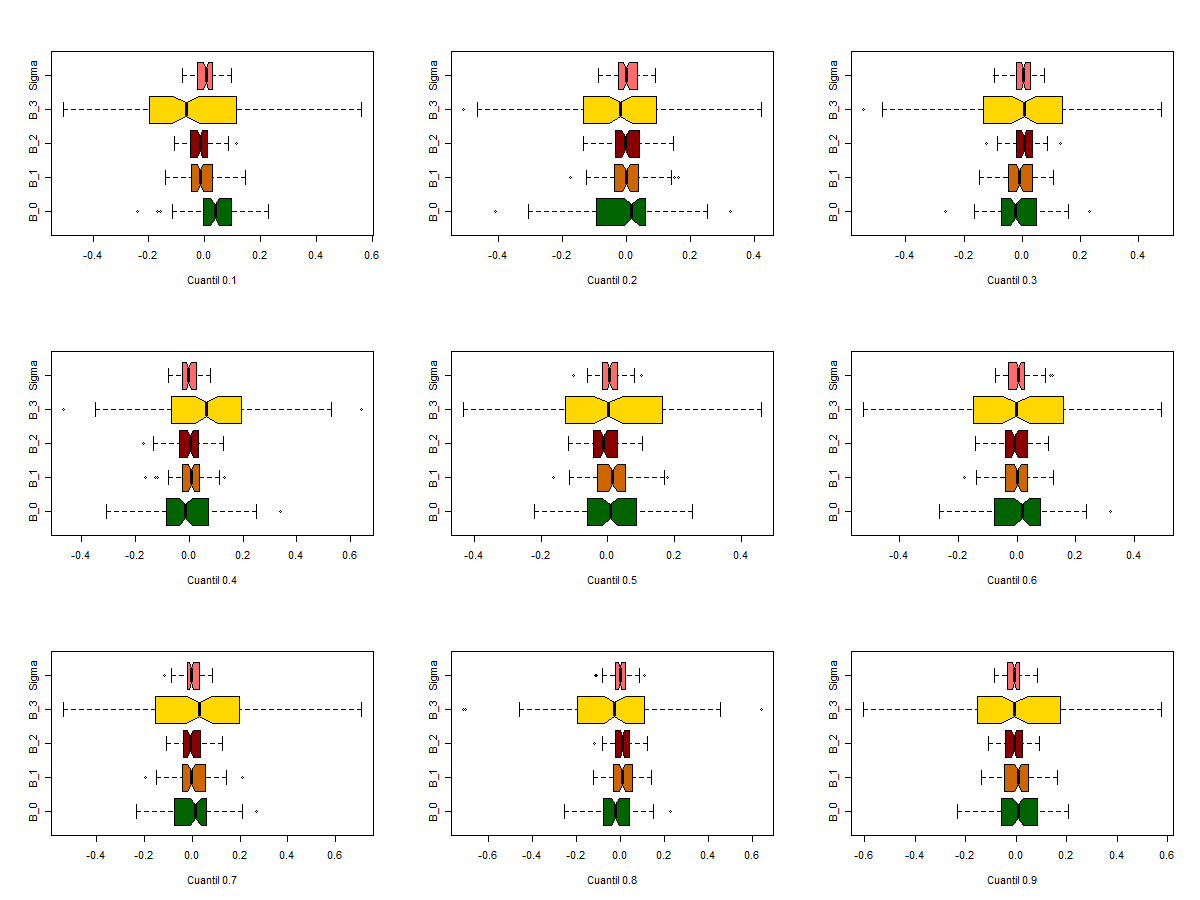
\includegraphics[width=\textwidth]{boxplot_simulacion}
	\caption{Valores de los parámetros (100 réplicas).}
\end{figure}

Por lo tanto, los resultados muestran que el método de estimación permite recuperar los parámetros pre-establecidos del modelo de regresión con censura intervalar.
